\documentclass[10pt,a4paper]{article}
\usepackage[margin=2.1cm]{geometry}
\usepackage{amsmath,amssymb,bm}
\usepackage{graphicx,booktabs,xcolor,enumitem,hyperref}
\hypersetup{colorlinks,linkcolor=blue!50!black,urlcolor=blue!50!black}
\newcommand{\note}[1]{\par\smallskip\noindent\colorbox{gray!12}{\parbox{\dimexpr\linewidth-2\fboxsep}{\small #1}}\par\smallskip}
\newcommand{\evd}[1]{\textsf{\small[#1]}}
\newcommand{\kc}{\kappa_2}
\newcommand{\simple}[1]{\par\noindent\textbf{In simple words:} #1\par\smallskip}
\title{TOP-Q --- Day 8 worked notes\\[2pt]\large Mach--Zehnder interferometers, meshes, and how errors add up}
\author{PH 5110 term paper --- Kotapati Kishore (EE26E016)}
\date{31 October 2026 (three days ahead of the revised plan)}
\begin{document}\sloppy\maketitle

\note{Labels as before. Everything here uses the \emph{same} sign convention as Days 1--6 ($d\bm a/dz=iH\bm a$), so the array results can be plugged in on Days 9--10. Simulations: 5 random target meshes $\times$ 1000 error samples per point. (Day 7 of the original plan was the buffer; numbering is kept.)}

\tableofcontents

%=====================================================================
\section{Building blocks}
%=====================================================================
\subsection{Directional coupler = a two-waveguide array \evd{Derived; Verified-by-test}}
Two identical guides coupled over a length $\ell$: $d\bm a/dz=i\kappa\sigma_x\bm a$, so
\[
B=e^{i\kappa\ell\sigma_x}=\begin{pmatrix}\cos\kappa\ell & i\sin\kappa\ell\\ i\sin\kappa\ell & \cos\kappa\ell\end{pmatrix}
=\begin{pmatrix}\sqrt\eta & i\sqrt{1-\eta}\\ i\sqrt{1-\eta} & \sqrt\eta\end{pmatrix},\qquad \eta=\cos^2\kappa\ell .
\]
$\eta$ = power that goes straight through (``bar''). 50:50 needs $\kappa\ell=\pi/4$. The test checks this equals the Day-5 propagator for a 2-guide array.
\textbf{Link to Day 3} \evd{Derived}: a gap error changes $\kappa$ by a fraction $\epsilon_\kappa$; at 50:50, $d\eta=-\sin(2\kappa\ell)\,\kappa\ell\,\epsilon_\kappa=-\tfrac{\pi}{4}\epsilon_\kappa$. So \textbf{coupler splitting error $\sigma_\eta=\tfrac{\pi}{4}\sigma_\kappa$} --- the same gap errors as on Day 3.

\subsection{Phase shifter}
$P(\phi)=\mathrm{diag}(e^{i\phi},1)$ on the top arm. On a chip this is usually a small heater: heating changes the effective index by $\Delta n$ over a length $L_h$, giving $\phi=\frac{2\pi}{\lambda}\Delta n\,L_h$. \textbf{Link to Days 4--6}: an unwanted propagation-constant error $\delta\beta$ in an arm of length $L$ is a phase error $\delta\phi=\delta\beta L$.

\subsection{The MZI \evd{Derived; Verified-by-test}}
$T(\theta,\phi)=B\,P(\theta)\,B\,P(\phi)$. Multiplying out the middle (ideal couplers):
\[
B\,P(\theta)\,B=i\,e^{i\theta/2}\begin{pmatrix}\sin\frac\theta2 & \cos\frac\theta2\\ \cos\frac\theta2 & -\sin\frac\theta2\end{pmatrix}
\ \Rightarrow\ |T_{11}|^2=\sin^2\tfrac\theta2\ (\text{bar}),\quad |T_{21}|^2=\cos^2\tfrac\theta2\ (\text{cross}).
\]
$\theta$ sets the \emph{split} (any ratio from 0 to 1); $\phi$ sets the \emph{relative phase} at the input. Every factor is unitary, so $T$ is unitary: no light is lost or created \evd{Verified-by-test, $\|T^\dagger T-\mathbb1\|<10^{-12}$}.
\simple{an MZI is a programmable beam splitter: one knob decides how the light divides, the other decides its phase.}

\subsection{Imperfect couplers limit the extinction \evd{Derived; Verified-by-test}}
With both couplers at $\eta\ne\tfrac12$:
$|T_{21}|^2=2\eta(1-\eta)(1+\cos\theta)$, so the \textbf{bar state is still perfect} ($\theta=\pi$ gives 0 cross), but the \textbf{cross state is not}: at most $4\eta(1-\eta)$. Simulated: 0.99 for $\eta=0.45$, 0.96 for $\eta=0.40$ (Fig.~\ref{fig:mesh}a). Correcting such imperfections by design is discussed by D.~A.~B.~Miller, ``Perfect optics with imperfect components'', \emph{Optica} (2015) \evd{Literature --- verify volume/page before citing}.

%=====================================================================
\section{Meshes}
%=====================================================================
Any $N\times N$ unitary can be built from $N(N-1)/2$ MZIs plus $N$ output phases. Reck \emph{et al.} (1994) used a triangle; Clements \emph{et al.}, \emph{Optica} \textbf{3}, 1460 (2016), doi:10.1364/OPTICA.3.001460, showed a \textbf{rectangular} layout with the same count but only $N$ columns and equal path lengths, which is more tolerant of loss \evd{Literature (verified bibliographic record)}. We use the rectangular layout (Fig.~\ref{fig:sch}). \textbf{Choice (stated):} we do not decompose a given target matrix; we draw random settings $\theta,\phi\in[0,2\pi)$ and treat the resulting clean mesh $U_0$ as the target. For small errors the results below do not depend on the settings.

\begin{figure}[h]\centering
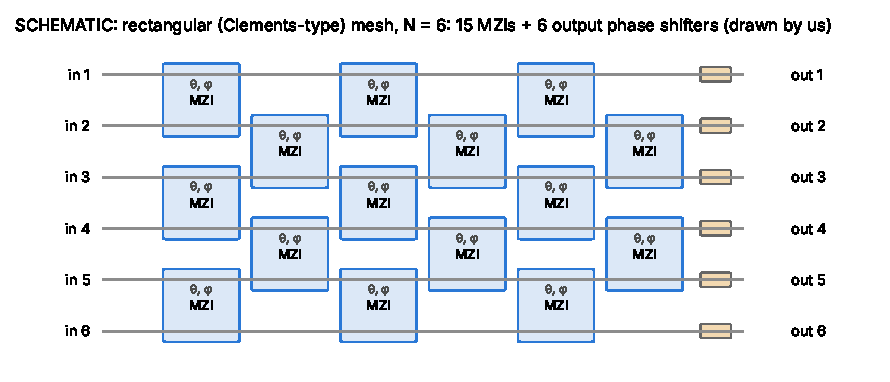
\includegraphics[width=0.85\linewidth]{../../figures/fig_mesh_schematic.pdf}
\caption{\textbf{Schematic drawn by us}, generated from \texttt{clements\_layout(6)}: 15 MZIs in 6 columns, then 6 output phase shifters.}
\label{fig:sch}
\end{figure}

\subsection{How good is a mesh? Two numbers}
\textbf{Normalised fidelity}
\[
F=\frac{|\mathrm{Tr}(U_0^\dagger U)|^2}{N\,\mathrm{Tr}(U^\dagger U)} .
\]
$F=1$ only if $U$ equals $U_0$ up to a global phase and a uniform loss; $F\le1$ always (Cauchy--Schwarz) \evd{Verified-by-test}.
\textbf{Output-intensity error}: for each single-port input, the fraction of light that ends up in the wrong output ports (total-variation distance), averaged over inputs. 0 = perfect, 1 = completely wrong.

%=====================================================================
\section{How errors add up \evd{Derived; Simulated}}
%=====================================================================
\subsection{Phase errors}
One phase error $\delta$ on one mode acts like $W=e^{i\delta P}$ ($P$ = projector on that mode inside the mesh). Then $\mathrm{Tr}\,W=N-1+e^{i\delta}$ and $|\mathrm{Tr}W|^2/N^2\approx1-(N-1)\delta^2/N^2$. Independent errors add their variances. A rectangular mesh has $N(N-1)$ internal/external phases plus $N$ output phases $=N^2$ phase shifters, so
\[
\boxed{1-F\approx(N-1)\,\sigma_\phi^2 .}
\]
\subsection{Coupler errors}
$B(\tfrac12+\epsilon)=B(\tfrac12)\,e^{-i\epsilon\sigma_x'}$ (a small extra rotation with eigenvalues $\pm1$), so $\mathrm{Tr}W=N-2+2\cos\epsilon$, giving $2\epsilon^2/N$ per coupler. With $N(N-1)$ couplers:
\[
\boxed{1-F\approx2(N-1)\,\sigma_\eta^2 .}
\]
\textbf{Check} (Fig.~\ref{fig:mesh}b,c): the simulated ratio to these formulas at small $\sigma$ is 0.99--1.01 for $N=4,6,8$, for both error types. They stay accurate up to $1-F\approx0.1$.

\begin{figure}[t]\centering
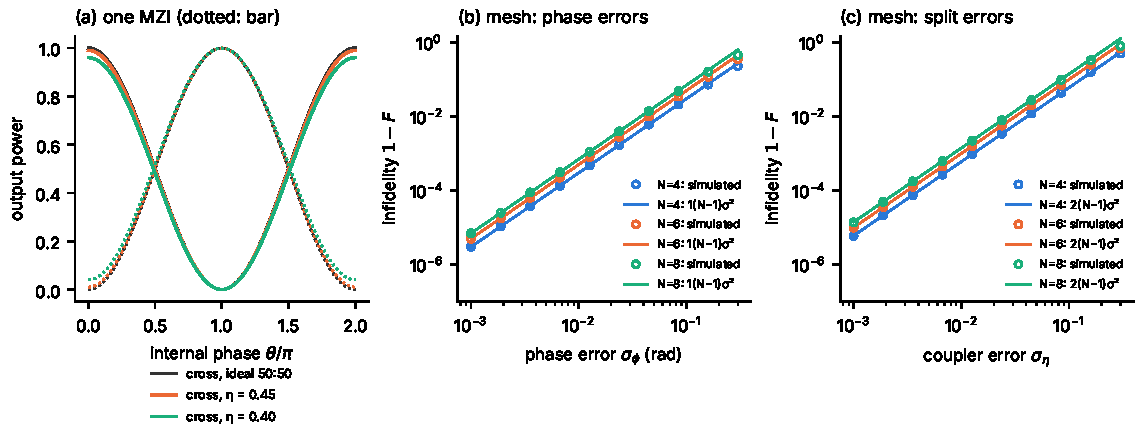
\includegraphics[width=\linewidth]{../../figures/fig_mzi_mesh.pdf}
\caption{\textbf{Simulation}, \texttt{scripts/day8\_mzi\_mesh.py} $\to$ \texttt{data/day8\_mzi\_mesh.npz}. (a) One MZI: cross (solid) and bar (dotted) power for ideal and imperfect couplers. (b,c) Mesh infidelity vs.\ error size: circles = simulation, lines = first-order formulas.}
\label{fig:mesh}
\end{figure}

\subsection{What these numbers mean}
\begin{itemize}[itemsep=1pt]
\item Infidelity grows like $\sigma^2$, but the \textbf{intensity error grows like $\sigma$}: for $N=8$, $\sigma_\phi=0.0126$~rad gives $1-F=0.001$ but 1.05\% of the light in wrong ports; $\sigma_\phi=0.045$ gives 1.4\% infidelity and 3.7\% misrouted light. \evd{Simulated}
\item To keep $F>0.99$ at $N=8$ you need $\sigma_\phi\lesssim0.038$~rad per phase shifter and $\sigma_\eta\lesssim0.027$ per coupler. \evd{Derived from the formulas}
\item \textbf{Compare with Day 6:} an array-based arm 10 coupling lengths long with on-site errors $\sigma_\beta=0.01\kc$ already has an arm-to-arm error of $\approx0.17$~rad --- more than four times this budget. Long arrays inside interferometer arms are therefore only sensible if their phase is protected, or if they are short. Days 9--10 test this properly.
\end{itemize}

%=====================================================================
\section{Hardware: real MZI meshes}
%=====================================================================
\textbf{Not ours.} The photos shown in our chat come from published work:
\begin{itemize}[itemsep=1pt]
\item The \textbf{programmable nanophotonic processor} of Shen \emph{et al.}, \emph{Nature Photonics} \textbf{11}, 441 (2017) --- a silicon chip of MZIs used as an optical neural network layer; its accuracy was limited by phase-setting errors (your reference [2]).
\item \textbf{Thermo-optic phase shifters}: metal heaters on top of silicon waveguides, wire-bonded to electronics; each heater sets one $\theta$ or $\phi$.
\end{itemize}
In such chips, the dominant errors are exactly the two we modelled: phase errors (heater calibration, thermal crosstalk, width errors in arms) and coupler errors (gap errors in the directional couplers). Cite the source papers shown with each image before reusing a photo.

\section{Code and tests}
New: \texttt{topq/mzi.py} (coupler, phase, MZI, embedding, Clements layout, mesh, random settings, fidelity, intensity error, unitarity error); \texttt{scripts/day8\_mzi\_mesh.py} (110~s). \texttt{tests/test\_mzi.py}: 23 tests, including the coupled-mode origin of the coupler, the closed form, the $4\eta(1-\eta)$ extinction limit, and both first-order fidelity laws. Suite: \textbf{119 passed}.

\section{Self-test}
\begin{enumerate}[itemsep=1pt]
\item Derive $B$ from the two-guide coupled-mode equation. What $\kappa\ell$ gives 50:50?
\item Why can a gap error be written as a splitting error $\sigma_\eta=\frac\pi4\sigma_\kappa$?
\item Show that $B P(\theta) B$ has bar power $\sin^2(\theta/2)$.
\item Why is the bar state still perfect with equal imperfect couplers, but the cross state is not?
\item Why does $1-F$ grow like $\sigma^2$ while the intensity error grows like $\sigma$?
\item For $N=8$, what phase error per shifter keeps $F>0.99$?
\end{enumerate}
\end{document}
